\documentclass[border=3pt]{standalone}
% Preâmbulo compartilhado pelos diagramas TikZ da aula 14 (SLAM com EIF)
\usepackage[T1]{fontenc}
\usepackage[utf8]{inputenc}
\usepackage{lmodern}
\usepackage{amsmath}
\usepackage{xcolor}
\usepackage{tikz}
\usetikzlibrary{arrows.meta,angles,quotes,decorations.pathmorphing,decorations.pathreplacing,calc,
                positioning,shapes.geometric,shapes.misc,backgrounds,fit,
                math}

% Paleta (mesma dos SVGs originais)
\definecolor{dblue}{HTML}{2A5B8C}
\definecolor{dorange}{HTML}{B3541E}
\definecolor{dgreen}{HTML}{4A7C59}
\definecolor{dred}{HTML}{9C4B4B}
\definecolor{dcream}{HTML}{F4F1EA}
\definecolor{dshade}{HTML}{DDD7C9}

% Função gaussiana (não normalizada por padrão de escala visual)
\pgfmathdeclarefunction{gauss}{3}{%
  \pgfmathparse{1/(#3*sqrt(2*pi))*exp(-((#1-#2)^2)/(2*#3^2))}%
}

% Estilos comuns (prefixo d... para não colidir com chaves internas do pgf)
\tikzset{
  >={Stealth[length=2mm]},
  dguide/.style={gray!55, dashed, line width=0.4pt},
  daxis/.style={gray!60, line width=0.7pt, ->},
  dbody/.style={fill=black!3, draw=black!80, line width=1pt},
  dacc/.style={draw=dblue, line width=1pt},
  dlbl/.style={black!55, font=\small},
  dsub/.style={black!45, font=\footnotesize},
  dstate/.style={circle, draw=black!80, fill=dcream, line width=1pt,
                 minimum size=17mm, font=\large, inner sep=1pt},
  dobs/.style={circle, draw=black!80, fill=dshade, line width=1pt,
               minimum size=14mm, font=\large, inner sep=1pt},
  dbox/.style={rounded corners=2pt, draw=black!80, fill=dcream, line width=1pt,
               align=center, inner sep=6pt},
  dop/.style={circle, draw=black!80, fill=white, line width=1pt,
              minimum size=6mm, inner sep=0pt, font=\small},
  dtrans/.style={->, dblue, line width=1pt},
  dmeas/.style={->, dorange, line width=1pt},
  dcurve/.style={line width=1pt, dblue},
  dcurveb/.style={line width=1.4pt, dorange},
}

\begin{document}
\hyphenpenalty=10000 \exhyphenpenalty=10000 \tolerance=9999 \emergencystretch=3em
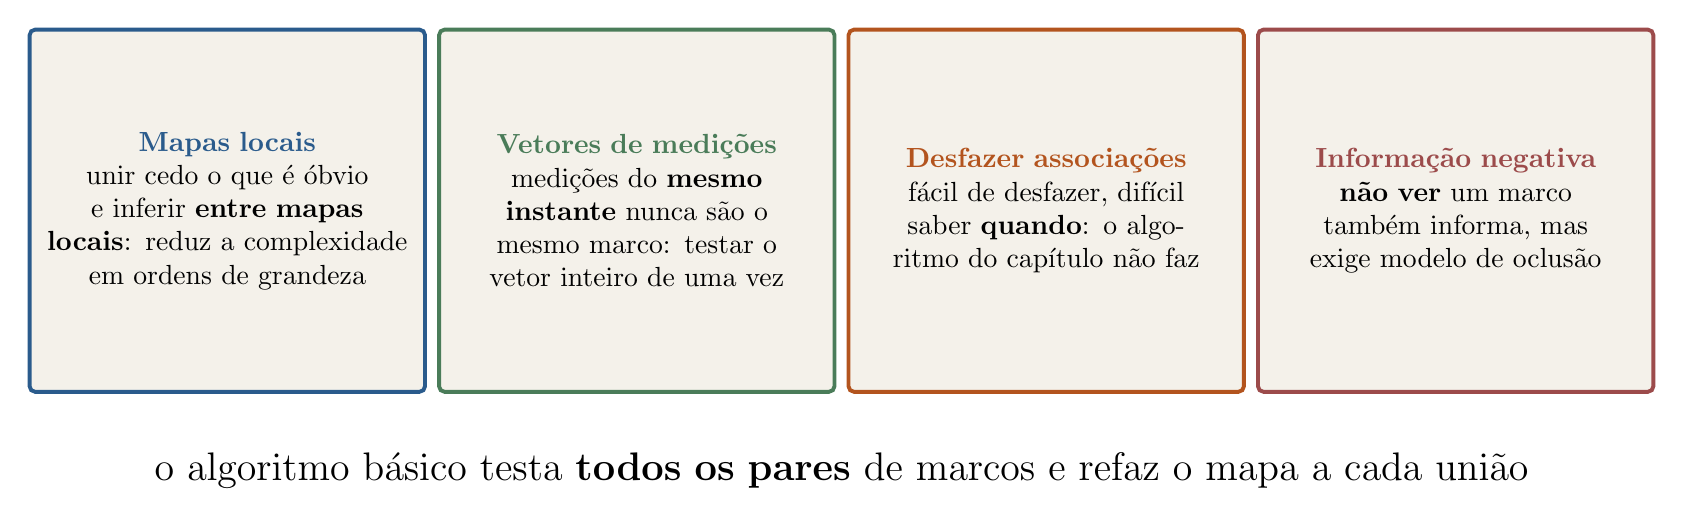
\begin{tikzpicture}[x=1cm,y=1cm]
\tikzset{c/.style={dbox, text width=4.6cm, minimum height=4.6cm, font=\normalsize, line width=1.4pt}}
\node[c, draw=dblue] at (0.0,0.0) {\textbf{\textcolor{dblue}{Mapas locais}}\\ unir cedo o que é óbvio e inferir \textbf{entre mapas locais}: reduz a complexidade em ordens de grandeza};
\node[c, draw=dgreen] at (5.2,0.0) {\textbf{\textcolor{dgreen}{Vetores de medições}}\\ medições do \textbf{mesmo instante} nunca são o mesmo marco: testar o vetor inteiro de uma vez};
\node[c, draw=dorange] at (10.4,0.0) {\textbf{\textcolor{dorange}{Desfazer associações}}\\ fácil de desfazer, difícil saber \textbf{quando}: o algoritmo do capítulo não faz};
\node[c, draw=dred] at (15.6,0.0) {\textbf{\textcolor{dred}{Informação negativa}}\\ \textbf{não ver} um marco também informa, mas exige modelo de oclusão};
\node[font=\Large, text width=19cm, align=center] at (7.8,-3.3) {o algoritmo básico testa \textbf{todos os pares} de marcos e refaz o mapa a cada união};
\end{tikzpicture}
\end{document}
